%!TEX root = volumeFinal.tex 
\chapter{\label{chap:planejamento}Planejamento automatizado}

Planejamento automatizado é uma sub-área da inteligencia artificial que estuda o processo de geração automática de planos. O processo para gerar um plano, é feito a partir da escolha e organização das ações, antecipando os resultados esperados das ações, em busca do seu objetivo. Um plano pode ser descrito como uma sequencia de ações que se forem executadas chegam a um objetivo \cite{ghallab2004automated}. O planejamento na computação se diferencia das outras áreas pelo fato de que todo o plano é gerado automaticamente \cite{intelligence2003modern}. 

\section{Representação do problema}
Uma entrada para qualquer técnica de planejamento é uma descrição do problema a ser resolvido. Isso é necessário para não precisar representar todos os estados e transição do problema. Com a descrição do problema os estados e transição não precisam ser explícitos, mas faz com que os estados não descritos possam ser computados \cite{ghallab2004automated}. Como foi visto no capitulo \ref{chap:agentes}, os estados são os estados para o agente se situar no ambiente e transições são para a interação com o ambiente. Um problema de planejamento pode ser descrito como \textit{P} = \textit{($\Sigma$, $s_{0}$, g)}. Onde \cite{ghallab2004automated}:

\begin{itemize}
	\item $\Sigma$- é a representação do problema;
	\item $s_{0}$- é o estado inicial, estado onde o problema começa;
	\item g- é o objetivo, estado onde o problema deve acabar.
\end{itemize}

Para representar o problema é necessário representar os estados do ambiente. Uma forma de fazer isso é utilizando lógica matemática. Sendo assim um estado do ambiente é representados por um conjunto de átomos que resultam em verdadeiro ou falso dependendo da interpretação do ambiente \cite{ghallab2004automated}. Vamos lembrar do problema do Capitulo \ref{chap:busca}, chegar a uma determinada cidade, estados para esse problema podem ser estar em determinada cidade e ter ligação entre as cidades, representado respectivamente como \textit{estar(cidade)} \textit{terLigação(cidadeOrigem, cidadeDestino)}.   

Além dos estados do ambiente precisamos determinar as transições, que alteram os estados. As transições utilizam ações e são representadas por operadores de planejamento que alteram os valores dos átomos presentes em determinado estado. Um operador de planejamento é definido como \textit{op} = (nome(\textit{op}), precondições(\textit{op}), efeitos(\textit{op})), onde cada elemento é definido como \cite{ghallab2004automated}: 

\begin{itemize}
	\item nome(\textit{op}) - É o nome do operador de planejamento e \textit{op} é o conjunto de todas as variáveis que irão aparecer qualquer parte do operador de planejamento.  
	\item precondições(\textit{op}) - \textit{op} é o conjunto de átomos ou átomos negativos que representa a precondição do operador de planejamento. 
	\item efeitos(\textit{op}) - \textit{op} é o conjunto de átomos ou átomos negativos que representa o efeito do operador de planejamento
\end{itemize}

No nosso exemplo, um operador de planejamento seria a mudança de uma cidade A para outra cidade B, que poderia ser representado como:
\begin{itemize}
	\item nome- mudarDeCidade(cidadeA, cidadeB);
	\item precondições- estar(cidadeA) $\wedge$ terLigação(cidadeA, cidadeB);
	\item efeitos- $\neg$ estar(cidadeA) \and estar(cidadeB).
\end{itemize}  

O nome deve ser único pelo proposito de o nome poder se referir ao operador por completo, ou seja, após definido apenas com o nome pode-se inferir as pré e pós condições, assim escrevendo o nome(\textit{op}) para se referir a todo o operador de planejamento \textit{op} \cite{ghallab2004automated}. 

O processo de geração do plano é feito pelo planejador, para isso ele utiliza a representação do problema, o estado inicial e os objetivos como entrada \cite{ghallab2004automated}. A figura \ref{fig:planmodelo} representa esse processo. 

\begin{figure}[ht]
	\centering
	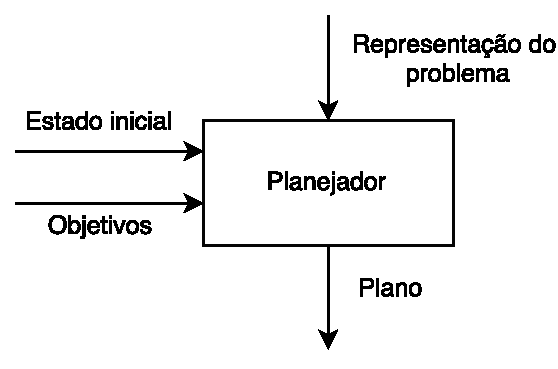
\includegraphics[width=0.4\textwidth]{fig/modelo.pdf}
	\caption{Problema de planejamento}
	\label{fig:planmodelo}
\end{figure} 

O domínio do problema é a parte do mundo que é expressada pelo conjunto de informações que é usado pelo planejador para gerar o plano \cite{intelligence2003modern}. No nosso exemplo, se representássemos as cidades presentes no mapa, apenas aquelas cidades seriam nosso domínio, e a única ação disponível no domínio seria mudar de cidade.

\msr[inline]{Falar mais de domínio? exemplos de domínios?}

\section{HTN} 

Dentro da área de planejamento existe o planejamento hierárquico, chamado de \textit{Hierarchical Task Network} (HTN). Em planejamento HTN as ações são tratadas em mais alto nível \cite{intelligence2003modern}. 

Além da representação do problema, um conjunto de métodos é adicionado como entrada, onde este conjunto serve para decompor as tarefas em tarefas menores. O planejamento é feito decompondo tarefas não primitivas recursivamente até chegar em tarefas primitivas, que podem ser realizadas com um operador de planejamento \cite{ghallab2004automated}. Um método HTN é definido como \textit{m} = (nome(\textit{m}), tarefa(\textit{m}), subtarefas(\textit{m}), limitação(\textit{m})), onde cada elemento é definido como \cite{ghallab2004automated}: 

\begin{itemize}
	\item nome(\textit{m}) - Nome do método, que deve ser único, e \textit{m} é o conjunto de variaveis que será utilizado em \textit{m}. 
	\item tarefa(\textit{m}) - É uma tarefa não primitiva.
	\item (subtarefa(\textit{m}),limitação(\textit{m})) - É uma ligação de tarefa de ligação.
\end{itemize}

Uma tarefa de ligação é definida como um par w = (U,C), onde U é um conjunto de tarefas de ligação e C um conjunto de limitações. Cada limitação deve ser satisfeita em todo o plano e cada tarefa de ligação é decomposta em sub tarefas até todas as tarefas se tornarem primitivas. 
Um exemplo de tarefa pode ser uma viagem de taxi, cada elemento poderia ser representado por:

\begin{itemize}
	\item nome- ViagemTaxi(de, para)
	\item tarefa- pegarTaxi
	\item (subtarefa({corrida(de, para), pagarTaxi}), distancia entre as cidades < 100) 
\end{itemize}

Com a definição de método, é preciso definir um problema de planejamento HTN, um problema é descrito como P = ($s_{0}$, w, O, M), onde $s_{0}$ é o estado inicial, w a tarefa de ligação inicial, O é um conjunto de operadores de planejamento, e M é um conjunto de métodos \cite{ghallab2004automated}. A ideia do planejamento HTN é através desta descrição, decompor o estado inicial com a tarefa de ligação inicial, e continuar decompondo as tarefas que restarem pelo conjunto de métodos, até só restarem tarefas primitivas. O plano é composto apenas por tarefas primitivas, começando pela tarefa w até chegar ao objetivo. Na busca pelo plano, o planejamento HTN começa planejando por um caminho, quando um caminho de resolução leva a um fim de linha é realizado um retrocesso(\textit{backtracking}) até um caminho que tenha uma possibilidade diferente de caminho do que foi tomado anteriormente \cite{intelligence2003modern}. 

\section{AHTN} 

\textit{Adversarial hierarchical-task network} (AHTN) é um algoritmo proposto para tentar solucionar o problema do grande fator de ramificação dos jogos em tempo real \cite{ontanon2015adversarial}. Nele são combinados técnicas de HTN com o algoritmo \textit{minimax search}. O algoritmo \ref{alg:ahtn} \cite{ontanon2015adversarial} é a representação da técnica de AHTN, e assume que existem dois jogadores, MAX e MIN, como no algoritmo de \textit{minimax search} apresentado no capitulo \ref{chap:busca}. 

\begin{algorithm}
	\caption{AHTNMax(s, $N_{+}$, $N_{-}$, $t_{+}$, $t_{-}$, d)}
	\label{alg:ahtn}
	\begin{algorithmic}[1]
		\If {terminal(s) $\vee$ d $\leq$ 0}
		\State	\Return ($N_{+}$, $N_{-}$, e(s))
		\EndIf
		\If {nextAction($N_{+}$, $t_{+}$) $\neq$ $\perp$}
		\State t = nextAction($N_{+}$, $t_{+}$) 
		\State \Return AHTNMin($\gamma$(s,t), $N_{+}$, $N_{-}$, t, $t_{-}$, d-1)
		\EndIf
		\State $N_{+}^{*}$ = $\perp$, $N_{-}^{*}$ = $\perp$, $v^{*}$ = $-\infty$
		\State $\aleph$ = $decompositions_{+}(s, N_{+}, N_{-}, t_{+}, t_{-})$
		\ForAll{$N \in \aleph$}
		\State $(N^{'}_{+}, N^{'}_{-}, v^{'}) = AHTNMax(s, N, N_{-}, t_{+}, t_{-}, d)$
		\If{$v^{'} > v^{*}$}
		\State $N_{+}^{*} = N^{'}_{+}, N_{-}^{*} = N^{'}_{-}, v^{*} = v^{'} $
		\EndIf
		\EndFor		
		\State \Return $(N_{+}^{*}, N_{-}^{*}, v^{*} )$
	\end{algorithmic}
\end{algorithm}

Cada nodo da arvore das jogadas é definido por uma tupla $(s, N_{+}, N_{-}, t_{+}, t_{-})$, onde s é o estado corrente do ambiente, $N_{+}$ e $N_{-}$ são a representação de planos HTN para os jogadores max e min, respectivamente, $t_{+}$ e $t_{-}$ representam ponteiros para qual parte do plano HTN está sendo executado, sendo  $t_{+}$ uma tarefa de $N_{+}$ e $t_{-}$ uma tarefa de $N_{-}$. 

A função \textit{nextAction(N,t)} faz com que, dado um HTN N e um ponteiro t, seja encontrada a tarefa primitiva que deve ser executada em N. Se N ainda não estiver completamente decomposto, ou seja, ainda existem tarefas não primitivas, então \textit{nextAction(N,t)} = $\perp$. Já $decompositions_{+}(s, N_{+}, N_{-}, t_{+}, t_{-})$ denota o conjunto das decomposições validas que adicionem apenas um novo método em $N_{+}$. A partir de uma função de avaliação, que pode ser aplicada sobre um estado, é retornado a recompensa de max em um estado terminal ou uma aproximação se o estado for não terminal.

A partir destas definições, o algoritmo para AHTNMin é análogo. O algoritmo retorna o melhor plano encontrado para os dois jogadores, e também o resultado da função de avaliação no nodo terminal alcançado após a execução dos planos. A grande diferença entre o algoritmo de AHTN e o algoritmo do \textit{minimax search}, é que as chamadas recursivas nem sempre se alternam entre max e min. O algoritmo troca de nodos max para min apenas quando os planos estão totalmente decompostos a ponto de gerar uma ação. 
